\subsection{Lückenerhaltende Reduktionen (GP-Reduktionen)}

\paragraph{Schwellwertproblem}
Liegt die optimale Lösung oberhalb oder unterhalb des Schwellwerts $t$?

\paragraph{Lückenproblem}
Liegt die optimale Lösung oberhalb oder unterhalb der Lücke $[s,c)$? D.h. ist $Opt < s \vee Opt \geq c$?
Falls Lösung in der Lücke: keine Aussage.

Siehe \emph{Promise-Problem}: Es ist garantiert dass die Eingabe nicht $Opt \in [s, c)$ hat.

\underline{Fallunterscheidung:} Sei $y$ die berechenbar Lösung.
TODO drawings
\begin{itemize}
    \item Fall 1: $y \geq c$ (oberhalb):
        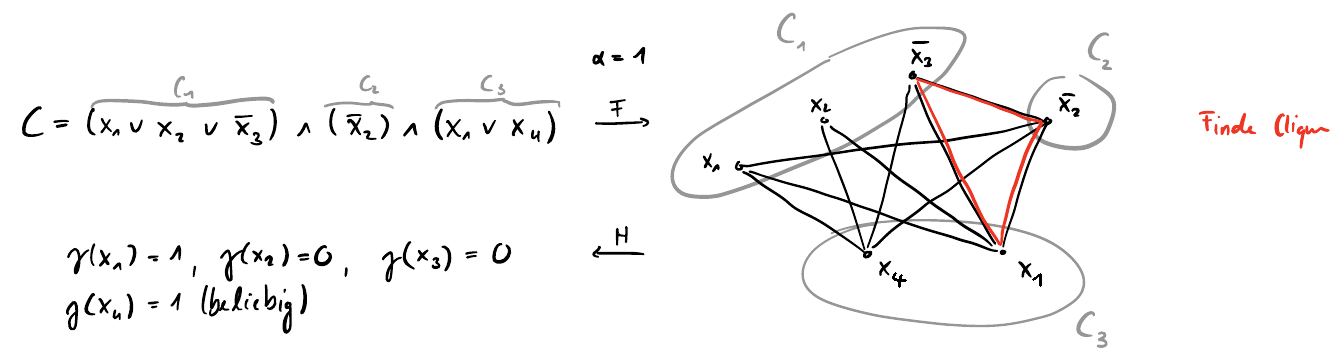
\includegraphics[width=0.2\textwidth]{images/ap-reduktion-beispiel.png}
        $\implies$ $Opt$ muss oberhalb liegen.
    \item Fall 2: $y < s$ (unterhalb):
        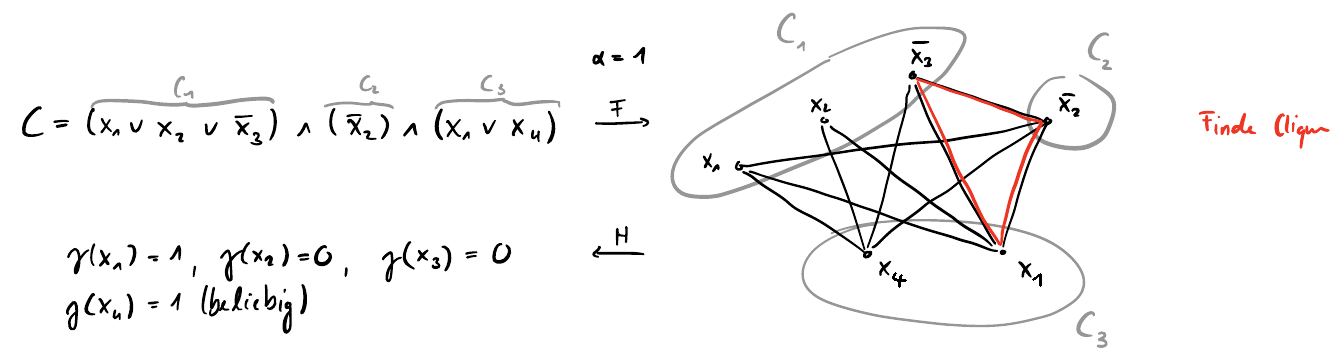
\includegraphics[width=0.2\textwidth]{images/ap-reduktion-beispiel.png}
        $\implies$ $Opt$ muss unterhalb liegen. \\
        Annahme: Approximation ist gut genug, so dass sie nicht über die Lücke geht.
    \item Fall 3: $y \geq s$ (innerhalb):
        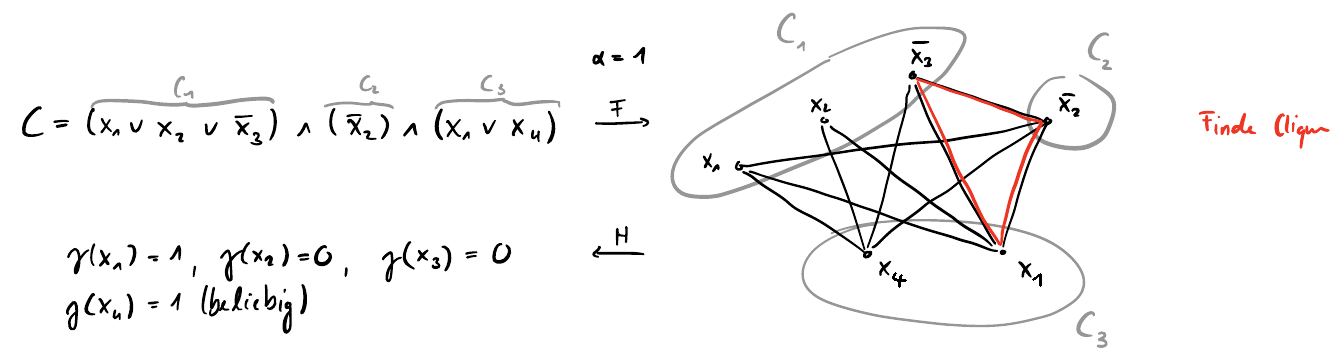
\includegraphics[width=0.2\textwidth]{images/ap-reduktion-beispiel.png}
        $\implies$ $Opt$ muss oberhalb liegen (kann nicht in der Lücke liegen).
\end{itemize}
In allen Fällen ist das Lückenproblem entscheidbar.
%
\begin{center}
    $\exists$ gute Approximation (kleine Lücke möglich) $\implies$ Lückenproblem entscheidbar

    Lückenproblem schwer $\implies$ $\not \exists$ gute Approximation
\end{center}
%
Beispiel:
Max-SAT ist selbst bei Lücke $ [s,c) = \left[ \frac{7}{8}, 1 \right) $ noch schwer.

\paragraph{Definition Lückenproblem GAP}
Sei $s, c\in \R^+, 0 \leq s \leq c \leq 1$.\footnote{Wir normalisieren auf $[0,1]$, siehe auch $|x|$ unten.}
Sei $U = (L, M, cost, goal) \in NPO$.
Das Lückenproblem $GAP_{s,c}(U)$ ist folgendes Entscheidungsproblem:

Eingabe:
$x \in L$ so dass $\frac{Opt_U(x)}{|x|} < s$ oder $\frac{Opt_U(x)}{|x|} \geq c$.
\\
Ausgabe:
JA, falls $\frac{Opt_U(x)}{|x|} \geq c$, sonst NEIN.

\paragraph{Lemma}
$GAP_{s,c}(U)$ NP-schwer ist $\implies$ $\not \exists$ polyzeit $\frac{c}{s}$-Approximation
für $U$ (falls P $\neq$ NP).

\underline{Beweis:}
Per Widerspruch. Nehme an es gäbe einen polyzeit $\frac{c}{s}$-Approximationsalgorithmus $A$.
OBdA sei $U$ ein Maximierungsproblem.
Zeige dass gilt:
$$ cost(A(x)) < s \cdot |x| \iff Opt_U(x) < s \cdot |x| $$
%
"$\Leftarrow$" : offensichtlich da $cost(A(x)) \leq Opt_U(x)$.

"$\Rightarrow$" : Nehme (für Widerspruch) an dass $Opt_U(x) \geq s \cdot |x|$.
Da die Lücke leer sein muss, gilt also $Opt_U(x) \geq c \cdot |x|$.
Ausserdem gilt per Definition von $\frac{c}{s}$-Approximation
$\frac{Opt_U(x)}{cost(A(x))} \leq \frac{c}{s}$.
Nun folgt ein Widerspruch:
$$ cost(A(x)) \geq \frac{s}{c} \cdot Opt_U(x) \geq \frac{s}{c} \cdot c \cdot |x| \geq s \cdot |x| $$

$\implies$ mit $A$ lässt sich $GAP_{s,c}(U)$ entscheiden. Widerspruch zu NP-schwer!

\paragraph{GP-Reduktion}
Seien $U_1, U_2$ Maximierungsprobleme.
Eine \emph{Lückenerhaltende Reduktion (gap-preserving reduction, GP-Reduktion)}
von $U_1$ zu $U_2$ mit Parametern $(s,c)$ und $(s',c')$ ist ein polyzeit Algorithmus $A$ mit:
\begin{enumerate}[label=(\roman*)]
    \item $ \forall x\in L_1 \cl A(x) \in L_2 $
    \item $ \frac{Opt_{U_1}(x)}{|x|} \geq c \implies \frac{Opt_{U_2}(A(x))}{|A(x)|} \geq c' $
    \item $ \frac{Opt_{U_1}(x)}{|x|} < s \implies \frac{Opt_{U_2}(A(x))}{|A(x)|} < s' $
\end{enumerate}

\underline{Bemerkung:}
Falls $\exists$ GP-Reduktion und $GAP_{s,c}(U_1)$ NP-schwer ist $\implies$ $GAP_{s',c'}(U_2)$ NP-schwer

$\implies$ untere Schranke $\frac{c}{s}$ für Approximation von $U_1$ $\implies$ untere Schranke
$\frac{c'}{s'}$ für Approx. von $U_2$

\underline{Motivation:} GP-Reduktion ist simpler als AP-Reduktion (nur ein Algorithmus).

\paragraph{Beispiel (MAX-E3SAT, MAX-2SAT)}
Eingabe: KNF-Formel. Ziel: Belegung finden die alle/möglichst viele Klauseln erfüllt.
\begin{itemize}
    \item \textbf{E3SAT}: exakt 3 verschiedene Literale pro Klausel
    \item \textbf{2SAT}: $\leq 2$ Literale pro Klausel, in P
    \item \textbf{MAX-2SAT}: NP-schwer
\end{itemize}

\paragraph{Lemma}
Für alle $a,b, \; a \neq 0, a \leq b$ existiert eine GP-Reduktion von MAX-E3SAT auf MAX-2SAT
mit Parametern $(a,b)$ und $\left( \frac{3}{5} + \frac{a}{10} , \frac{3}{5} + \frac{b}{10} \right)$.
\footnote{D.h. die Lücke/Approximation wird etwas schlechter.}

\underline{Beweis:}
Sei $C = C_1 \wedge ... \wedge C_m$ eine MAX-E3SAT-Instanz mit Klauseln
$C_i = l_{i1} \vee l_{i2} \vee l_{i3}$ und Variablen $x_1, ..., x_n$.

Konstruiere MAX-2SAT-Instanz: $\Phi_C = \bigwedge_{i=1}^m \Phi(C_i)$ mit zusätzlichen Variablen
$y_1, ..., y_m$ und mit
\begin{align*}
\Phi(C_i) &= (l_{i1}) \wedge (l_{i2}) \wedge (l_{i3}) \\
    & \wedge (\overline{l_{i1}} \vee \overline{l_{i2}}) \wedge (\overline{l_{i1}} \vee \overline{l_{i3}}) \wedge (\overline{l_{i2}} \vee \overline{l_{i3}}) \\
    & \wedge (l_{i1} \vee \overline{y_i}) \wedge (l_{i2} \vee \overline{y_i}) \wedge (l_{i3} \vee \overline{y_i}) \\
    & \wedge (y_i)
\end{align*}

Restlicher Beweis siehe Buch S.327.
Idee: für jede Belegung $\alpha$ für $C$ kann man $y_i$ so wählen dass $\leq 7$ der 10 Klauseln
erfüllt werden.

\paragraph{Lemma (Max-CLIQUE)}
Max-CLIQUE kann GP-reduziert werden auf Max-CLIQUE mit Parametern
$(\alpha, 1-\varepsilon), \; (\alpha^2, (1-\varepsilon)^2)$
für alle $\alpha \in (0, 1-\varepsilon), \; \varepsilon \in (0, \frac{1}{2})$.

\underline{Beweis:}
Sei $G=(V,E), \; |G|=|V|$.
Konstruiere $G \times G = ( V_{G \times G}, E_{G \times G} )$ mit
\begin{itemize}
    \item $V_{G \times G} = V \times V$
    \item $E_{G \times G} = \left\{ \{ (v,u) , (r,s) \} \st v,u,r,s \in V \text{ und }
    ( ( v=r , \{u,s\} \in E) \text{ oder } (\{v,r\} \in E) ) \right\}$
\end{itemize}

$Opt_{Max-CLIQUE}(G)$ = Clique der Grösse $k$ in $G$ $\implies$ Clique der Grösse $k^2$ in $G \times G$.

Fallunterscheidung:
\begin{itemize}
    \item $ Opt_{Max-CLIQUE}(G) < a \cdot |G| \implies
        Opt_{Max-CLIQUE}(G \times G) < a^2 \cdot |G|^2 = a^2 \cdot |G \times G|$
    \item $ Opt_{Max-CLIQUE}(G) \geq (1-\varepsilon) \cdot |G| \implies
        Opt_{Max-CLIQUE}(G \times G) \geq (1-\varepsilon)^2 \cdot |G|^2 = (1-\varepsilon)^2 \cdot |G \times G|$
\end{itemize}

\underline{Implikation:}

Jede konstante $c$-Approximation lässt sich iterativ verbessern (von $c$ auf $\sqrt{c}$, für $c>1$). \\
$\implies$ \emph{entweder} Max-CLIQUE $\in$ PTAS \emph{oder} Max-CLIQUE $\noindent$ APX
(= nicht konstant approximierbar).

Max-SAT $\leq_{AP}$ Max-CLIQUE (siehe \autoref{sec:ap-reduktionen}) und Max-SAT ist APX-vollständig
\footnote{Nicht in Vorlesung bewiesen} \\
$\implies$ Max-CLIQUE $\notin$ APX

TODO Beispiel Graphik
